%%%%%%%%%%%%%%%%%%%%%%%%%%%%%%%%%%%%%%%%%
% baposter Poster
% LaTeX Template
% Version 1.0 (15/5/13)
%
% Created by:
% Brian Amberg (baposter@brian-amberg.de)
%
% This template has been downloaded from:
% http://www.LaTeXTemplates.com
%
% License:
% CC BY-NC-SA 3.0 (http://creativecommons.org/licenses/by-nc-sa/3.0/)
%
%%%%%%%%%%%%%%%%%%%%%%%%%%%%%%%%%%%%%%%%%

%----------------------------------------------------------------------------
%	PACKAGES AND OTHER DOCUMENT CONFIGURATIONS
%----------------------------------------------------------------------------

\documentclass[a0paper,landscape,fontscale=0.385]{baposter}

\usepackage[font=small,labelfont=bf]{caption} % Required for specifying captions to tables and figures
\usepackage{booktabs} % Horizontal rules in tables
\usepackage{enumitem} % To change spacing in itemize and enumerate lists
\usepackage{multicol}
\usepackage{relsize} % Used for making text smaller in some places
\usepackage{amsfonts, amsmath, amsthm, amssymb} % For math fonts, symbols and environments
\usepackage{wrapfig} % Allows wrapping text around tables and figures
\usepackage[export]{adjustbox}% http://ctan.org/pkg/adjustbox
\usepackage{palatino} % Uncomment to use the Palatino font
\usepackage{graphicx} % Required for including images
\usepackage{graphbox}
\usepackage{mathtools}
\usepackage{colortbl}

\graphicspath{{figures/}} % Directory in which figures are stored

\definecolor{white}{RGB}{255,255,255}
\definecolor{cardinalred}{cmyk}{0.0,1.00,0.65,0.34}

\newenvironment{Figure}
  {\par\medskip\noindent\minipage{\linewidth}}
  {\endminipage\par\medskip}

\DeclarePairedDelimiterX{\norm}[1]{\lVert}{\rVert}{#1}
\DeclareMathOperator{\Tr}{Tr}

\begin{document}

\begin{poster}{
    columns=6,
    headerheight=0.10\textheight,
    borderColor=white, % Border color of content boxes
    headerColorOne=cardinalred, % Background color for the header in the content boxes (left side)
    headerColorTwo=cardinalred, % Background color for the header in the content boxes (middle)
    headerFontColor=white, % Text color for the header text in the content boxes
    boxColorOne=white, % Background color for the content in the content boxes
    headershape=roundedright, % Specify the rounded corner in the content box headers
    headershade=plain, % Specify the type of shading to be applied to the header boxes
    headerfont=\Large\sf\bf, % Font modifiers for the text in the content box headers
    textborder=rectangle,
    background=none,
    headerborder=open, % Change to closed for a line under the content box headers
    boxshade=none,
}
{}
%
%----------------------------------------------------------------------------
%	TITLE AND AUTHOR NAME
%----------------------------------------------------------------------------
%
{\sf\bf %
Early life adversity and white matter development %
in the Healthy Brain Network dataset
\hfill %
\null %
} % Poster title
{%
    \vspace{0.4em}
    Adam Richie-Halford\textsuperscript{1, 2}, %
    Ethan Roy\textsuperscript{2}, %
    John Kruper\textsuperscript{3}, %
    Jason Yeatman\textsuperscript{1, 2}, %
    Ariel Rokem\textsuperscript{3} \hfill \null \\
    {\smaller%
        1. Developmental-Behavioral Pediatrics, Stanford University, %
        2. Graduate School of Education, Stanford University, %
        3. Department of Psychology and eScience Institute, University of Washington %
        \hfill \null
    }
} % Author affiliations and email addresses
{%

\includegraphics[align=c,height=2.00cm]{logos/stanford_logo.png}%
\hspace{0.25em}

\includegraphics[align=c,height=1.85cm]{logos/UWlogo.png}%
} % University/lab logos

%----------------------------------------------------------------------------
%	INTRODUCTION
%----------------------------------------------------------------------------

\headerbox{Introduction}{name=introduction,column=0,row=0,span=2}{

\begin{itemize}[nosep, leftmargin=*]
    \item Early life adversity (ELA) comprises negative environmental
    experiences that require significant adaptation by an average child.
    \item ELA is associated with depression, PTSD, low educational
    attainment, and deficits in language development and executive
    functioning\cite{guloksuz2018exposome}.
\end{itemize}

\vspace{0.5em}
\noindent\textbf{%
    \underline{Question}: %
    How does early life adversity alter children's developing white matter, as
    assessed through diffusion MRI (dMRI)?
}
\vspace{0.5em}

\begin{itemize}[nosep, leftmargin=*]
    \item There is some evidence that children exposed to adversity exhibit
    differences in the uncinate fasciculus, cingulum, and superior longitudinal
    fasciculus\cite{gur2019burden}. 
    \item We sought to test these findings in \textbf{tract profile} analysis of
    dMRI data from 1,817 participants in the Healthy Brain Network
    study\cite{richiehalford2022analysis}, a large, heterogeneous dataset.
\end{itemize}

\vspace{-1em}
\begin{multicols}{4}
    \begin{Figure}
        \centering
        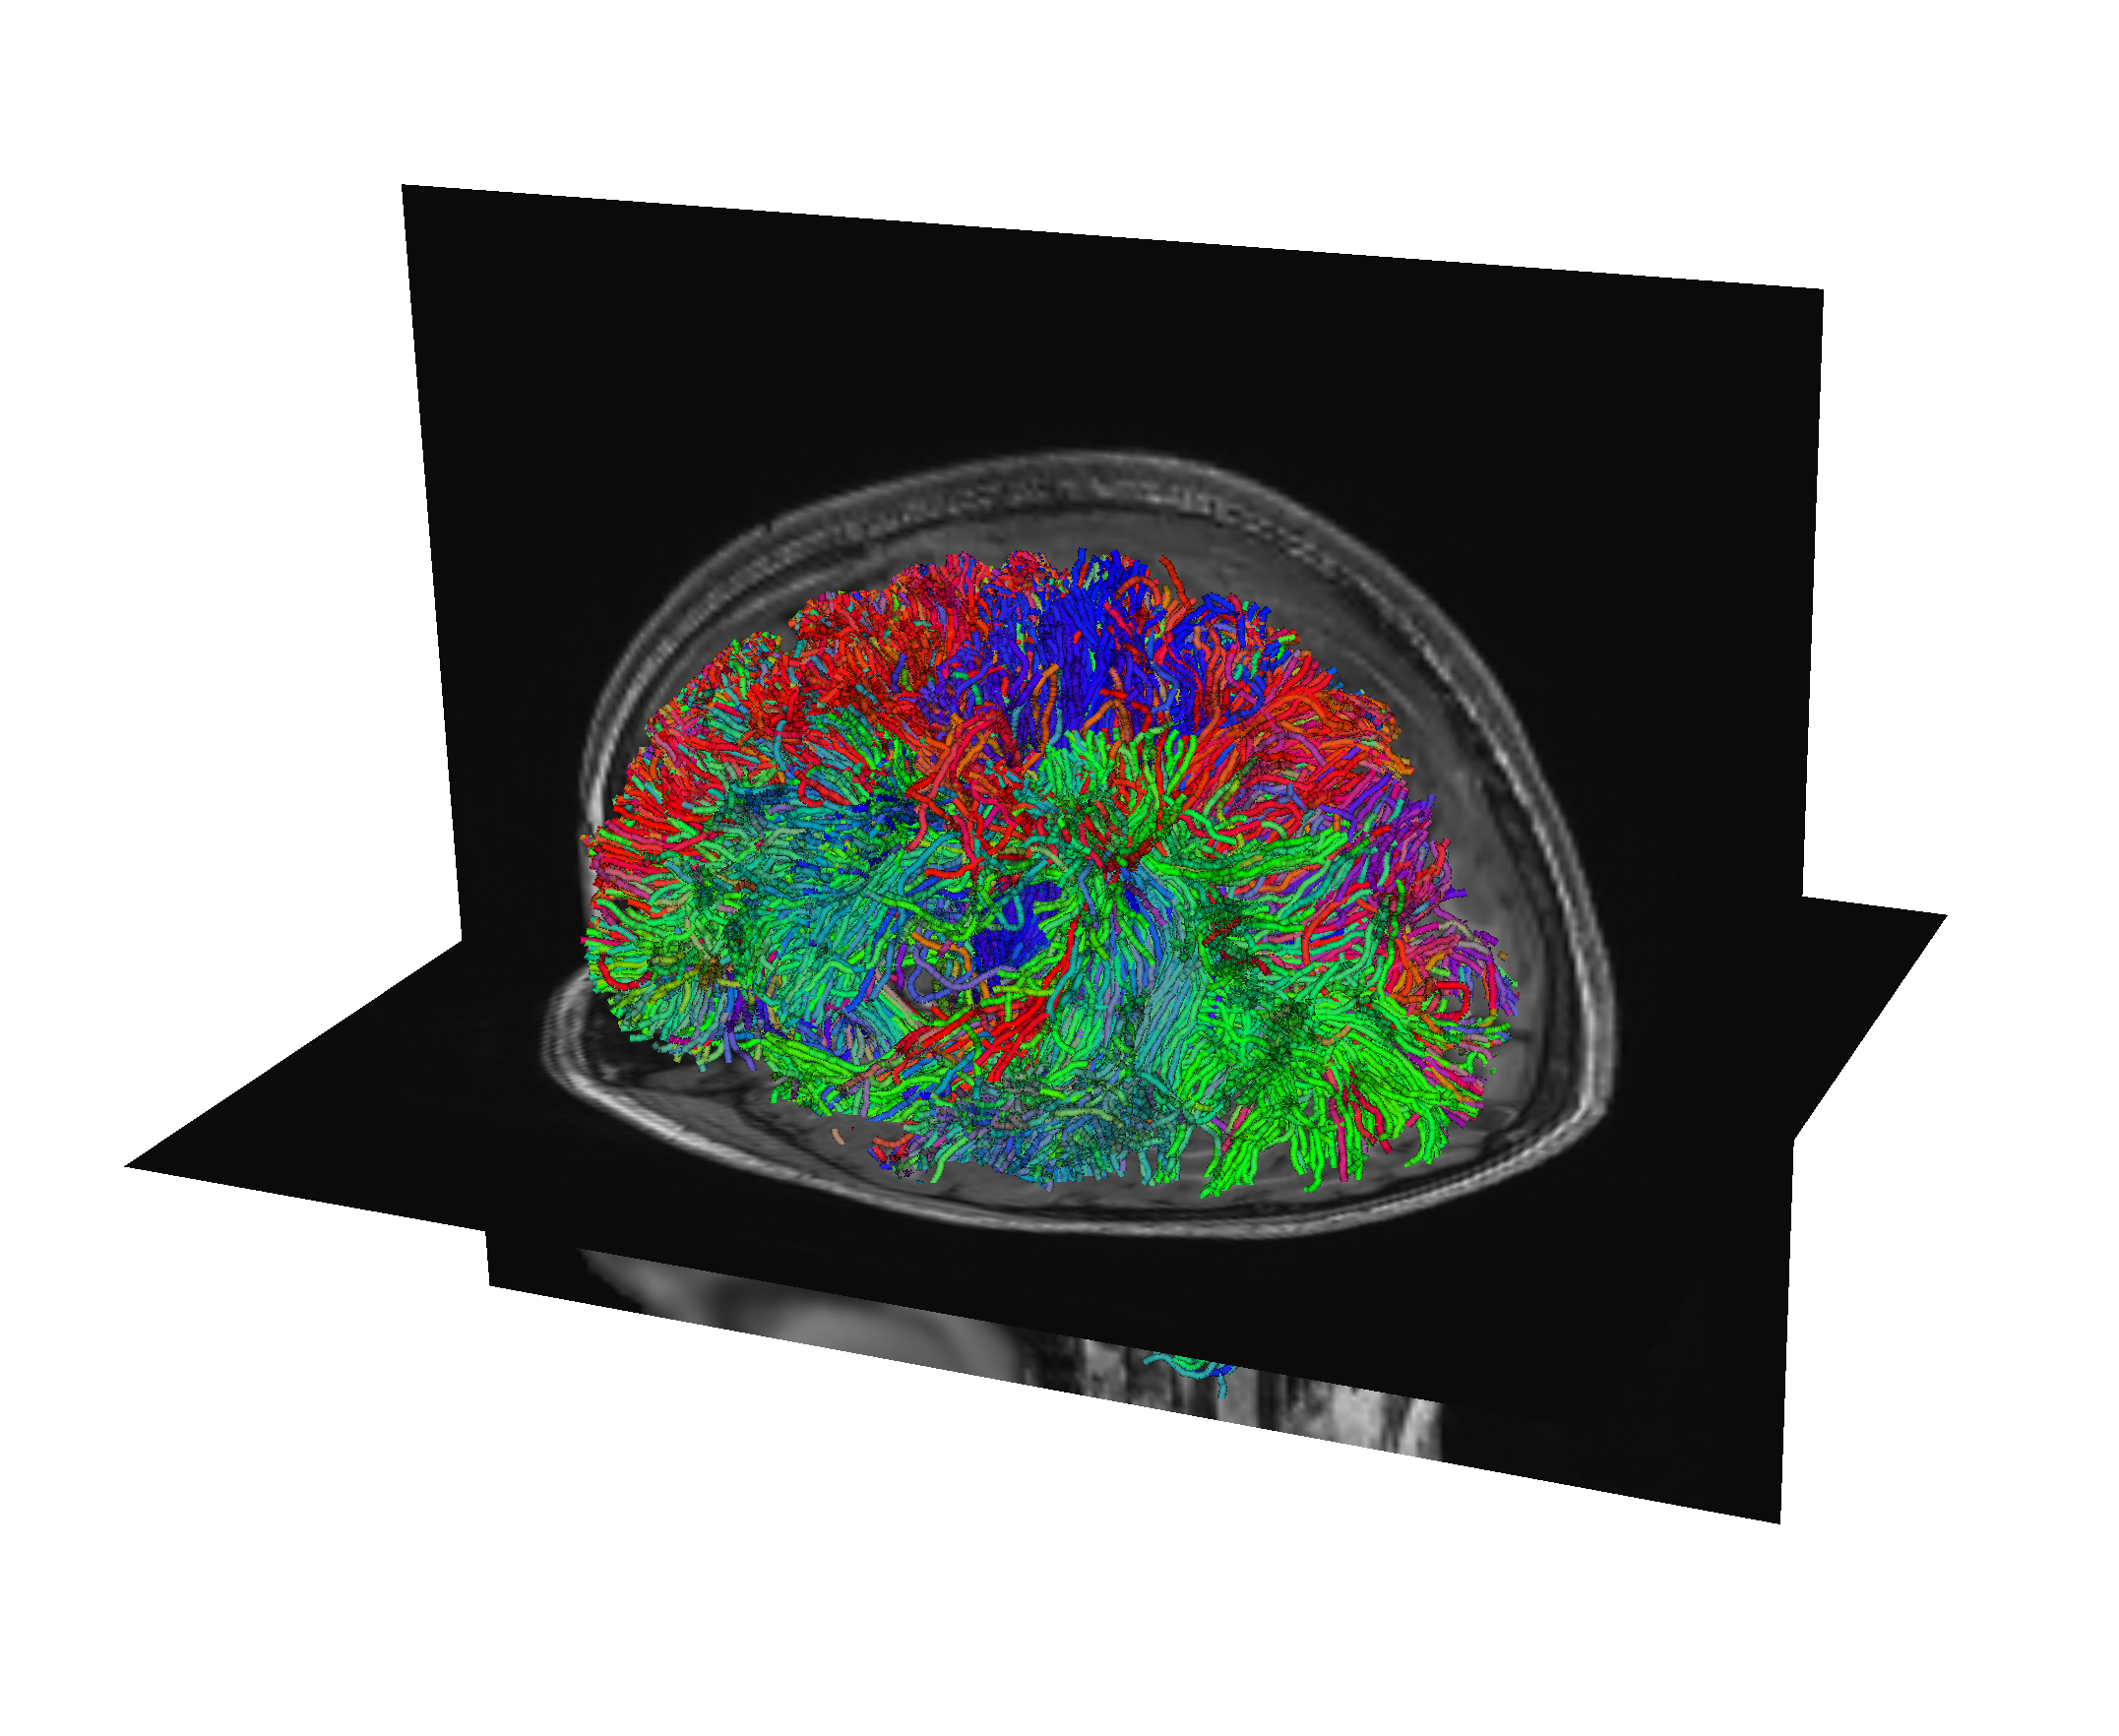
\includegraphics[width=1.0\linewidth]{whole_brain_trk.png}
        Whole brain tractography
    \end{Figure}
    \columnbreak
    \begin{Figure}
        \centering
        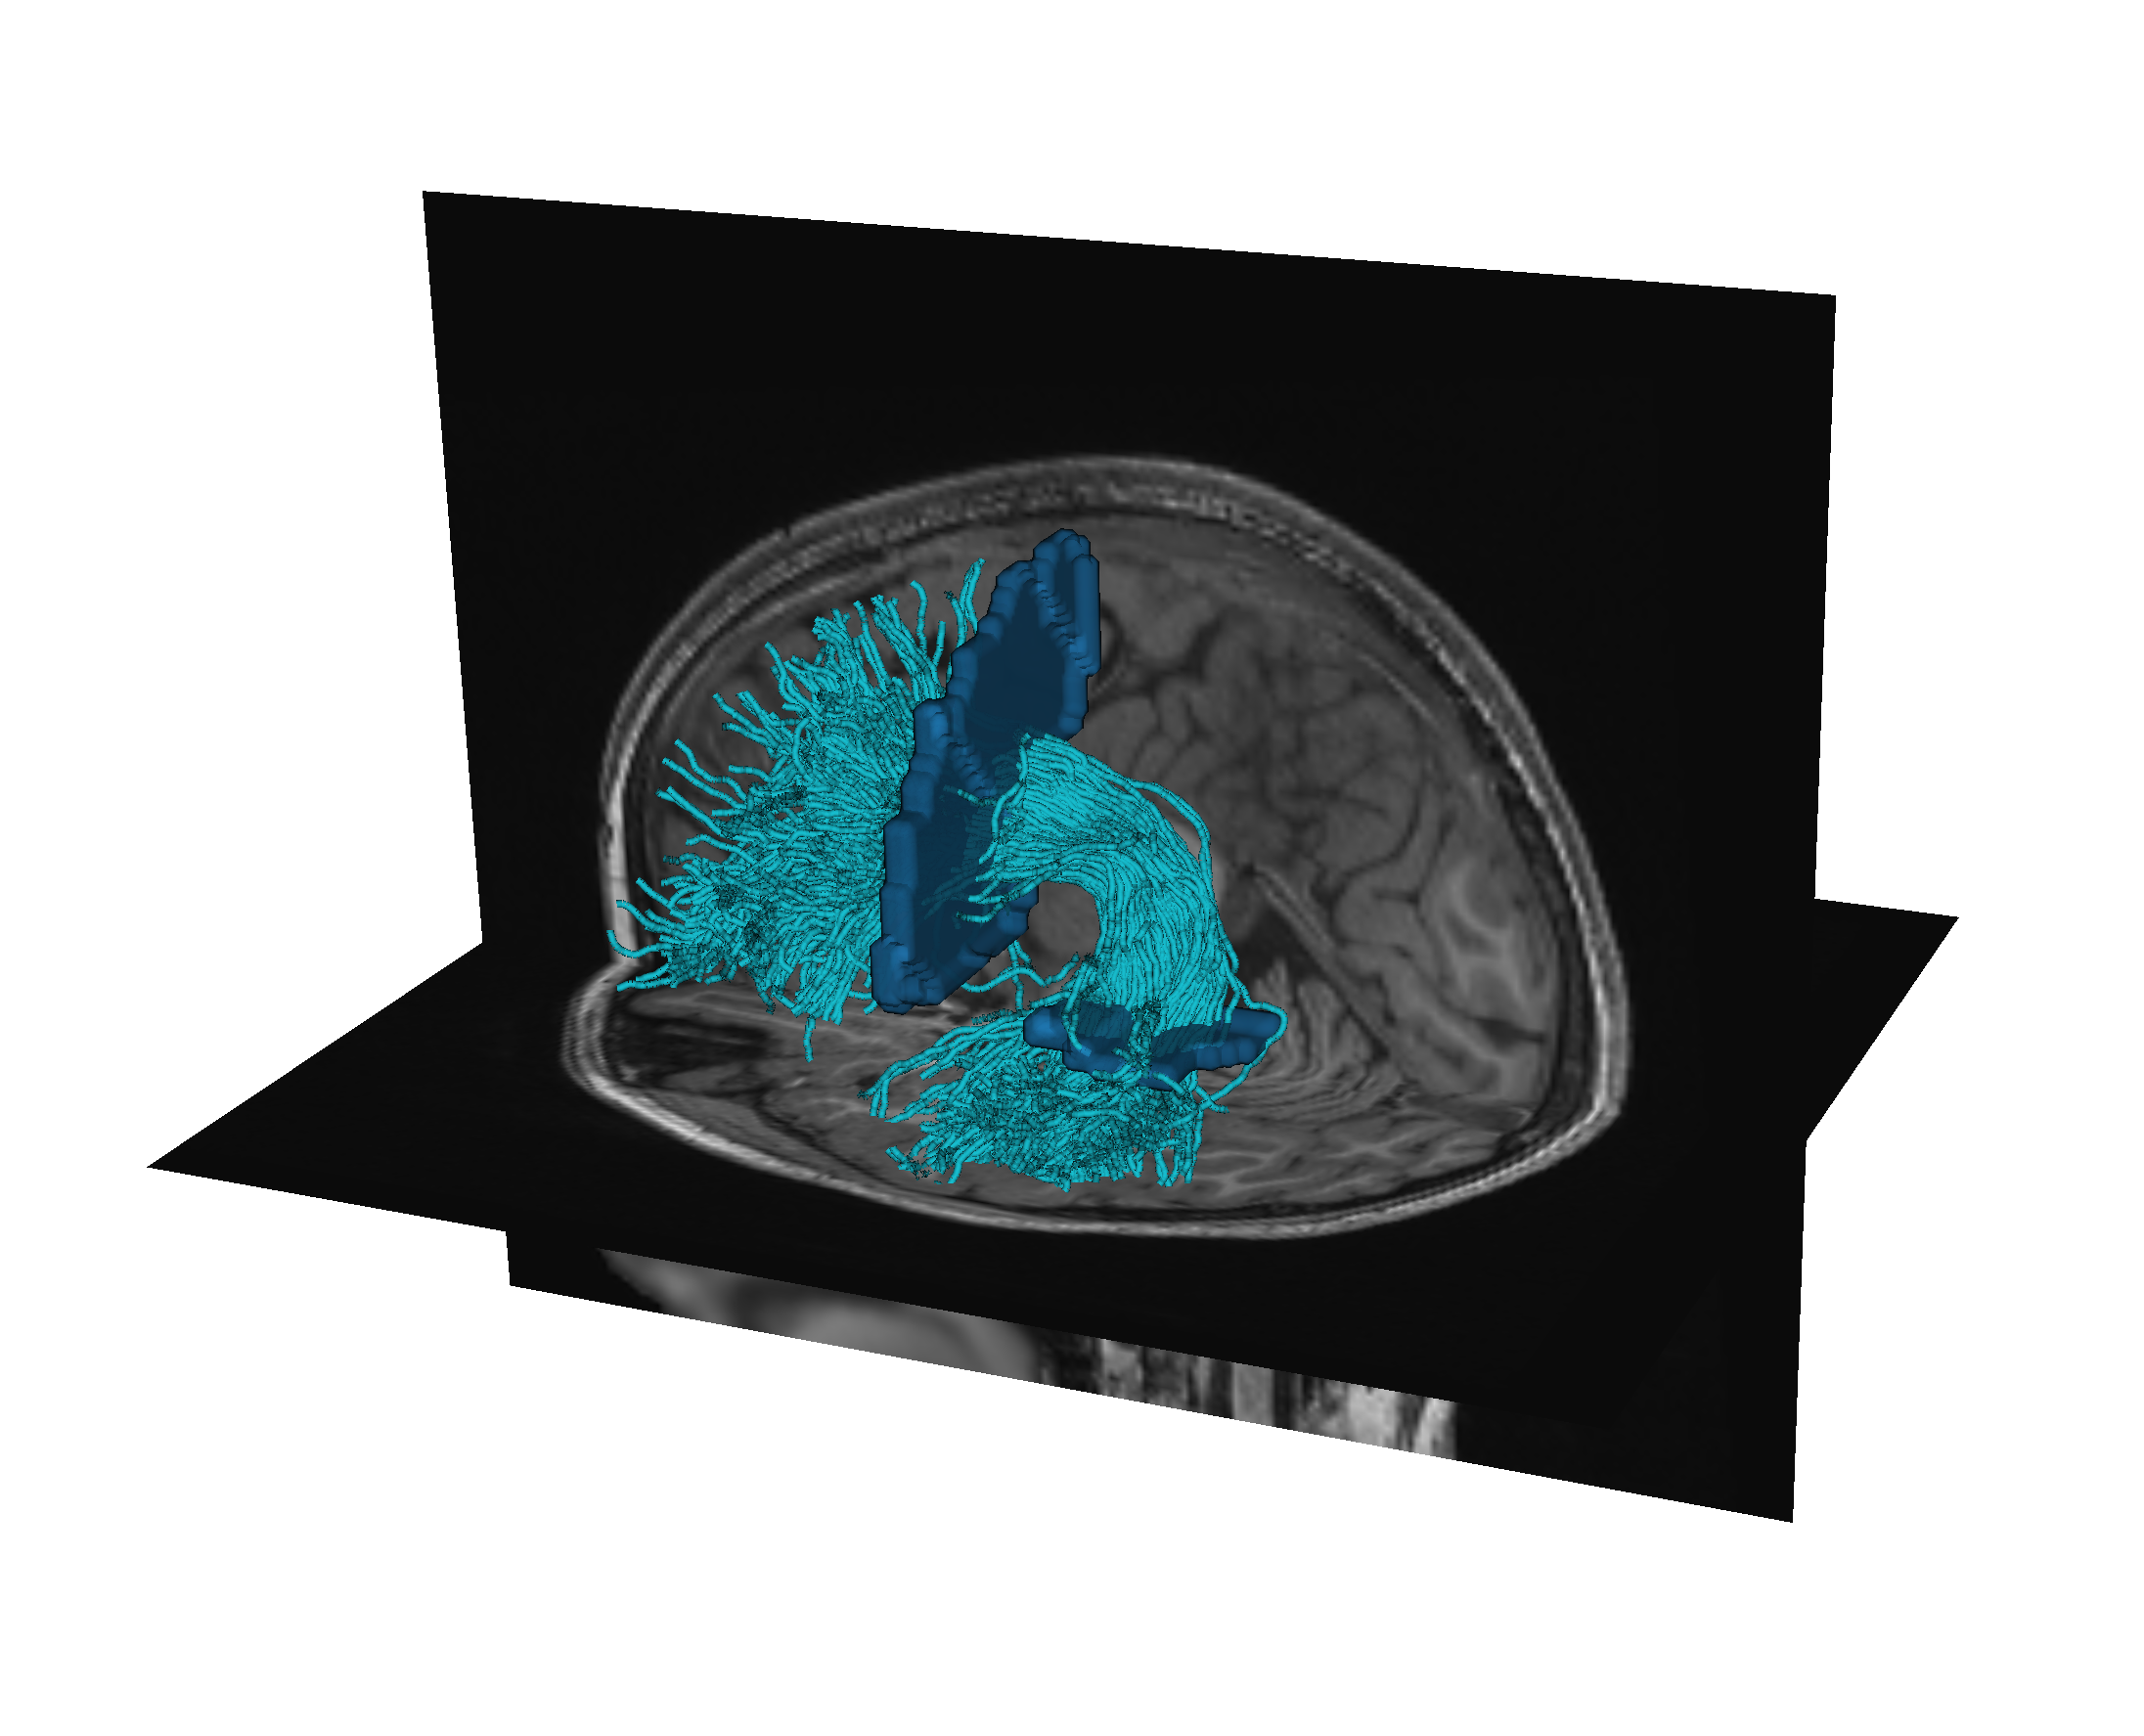
\includegraphics[width=1.0\linewidth]{arc_trk.png}
        Selecting a bundle with ROIs
    \end{Figure}

    \columnbreak
    \begin{Figure}
        \centering
        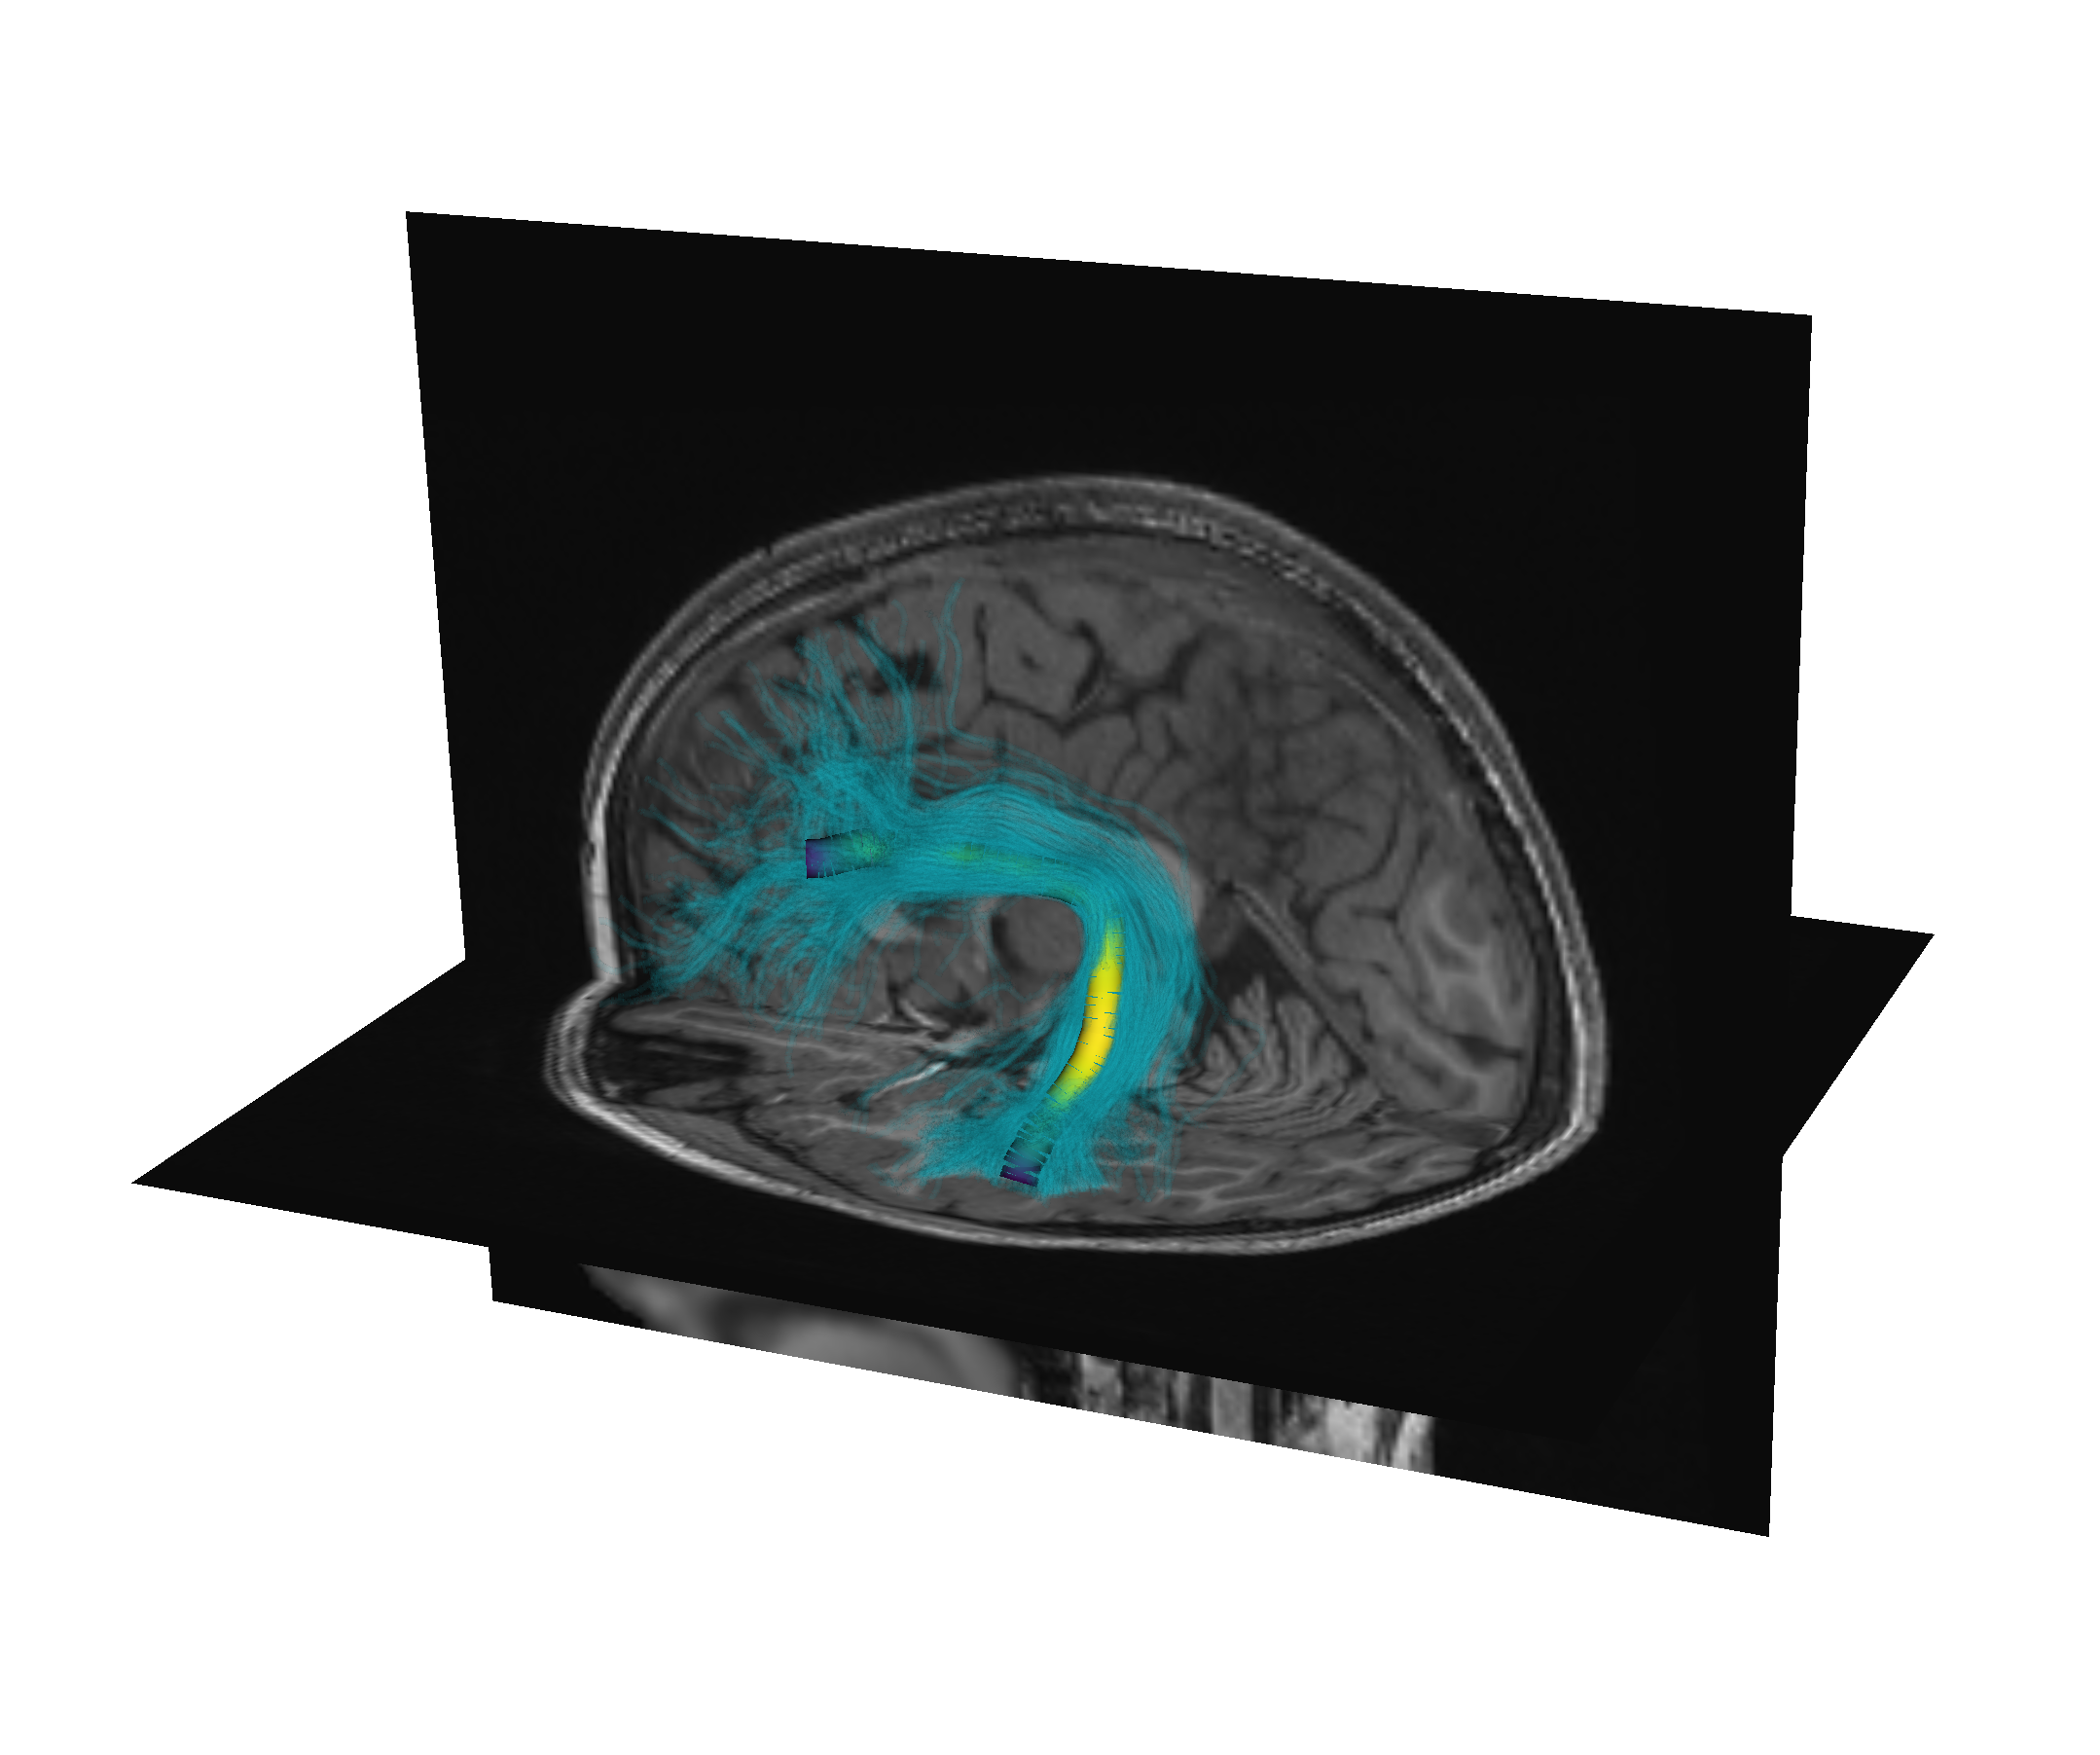
\includegraphics[width=1.0\linewidth]{arc_profile_trk.png}
        Extracting values along the length of the tract
    \end{Figure}
    \columnbreak
    \begin{Figure}
        \vspace{0.25cm}
        \centering
        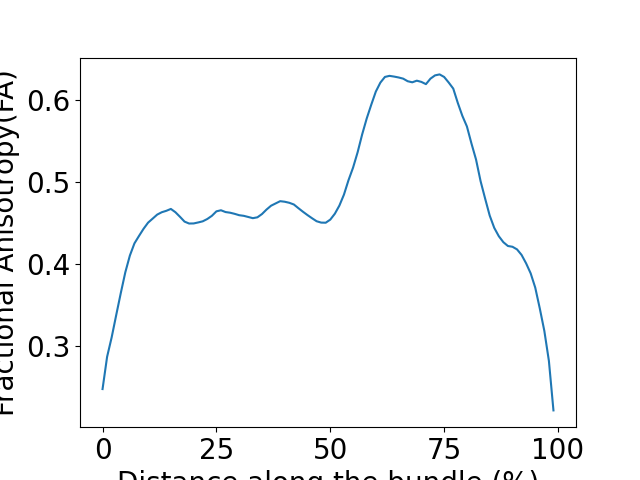
\includegraphics[width=1.0\linewidth]{tract_profile.png}
        Tract profile
    \end{Figure}

    \vspace{2em}
\end{multicols}
\vspace{-0.5em}
}

%----------------------------------------------------------------------------
%	RESULTS
%----------------------------------------------------------------------------

\headerbox{Results}{name=results,row=0,column=2,span=4}{

\begin{minipage}[b]{0.5\textwidth}
    \begin{center}
        No differences found between statistically matched ELA groups (p>0.05, FDR corrected for multiple comparisons)
    \end{center}

    \vspace{-1em}

    \begin{Figure}
        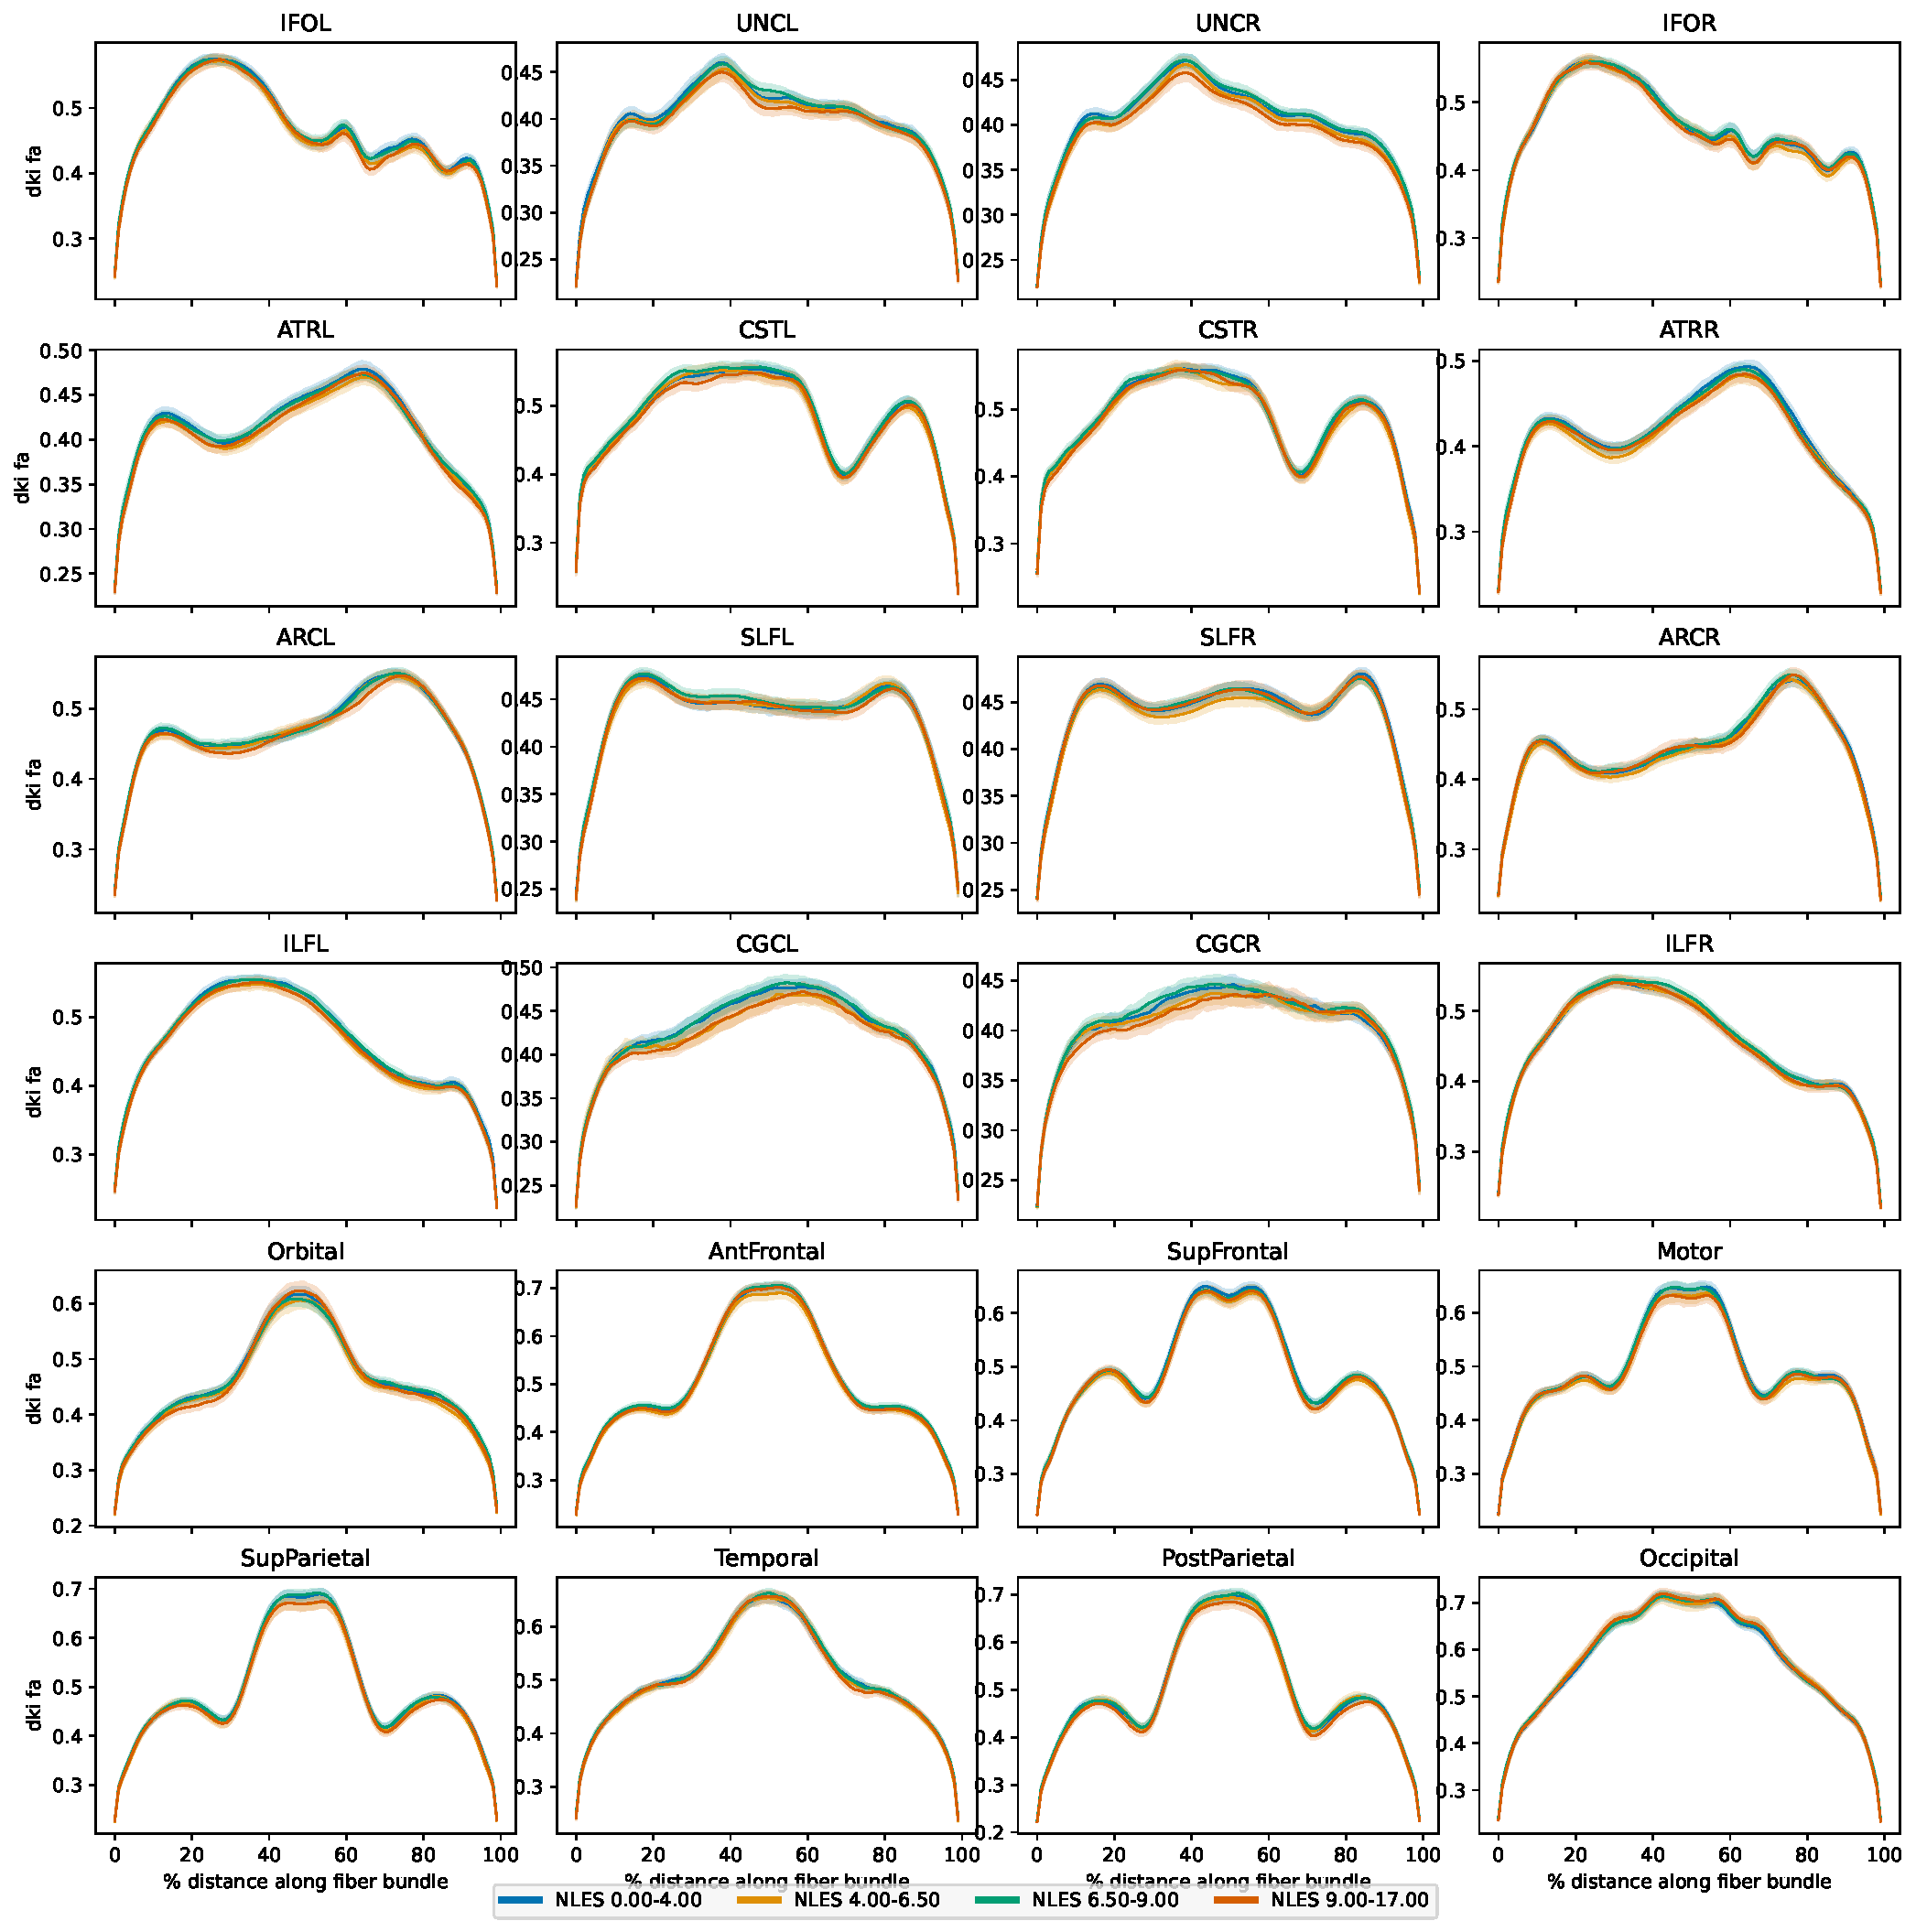
\includegraphics[width=\textwidth]{nles_tract_profiles_fa.pdf}
        \captionof{figure}{
            FA bundle profiles show no group differences between NLES quartiles.
            The $x$-axis is distance along the bundle. Error bands are
            95\% confidence intervals. Bundle abbreviations have a
            trailing “L” or “R” for the hemisphere. Bundle abbreviations:
            inferior fronto-occipital fasciculus (IFO), uncinate (UNC), anterior
            thalamic radiation (ATR), corticospinal tract (CST), arcuate fasciculus
            (ARC), superior longitudinal fasciculus (SLF). inferior longitudinal
            fasciculus (ILF), cingulum cingulate (CGC), orbital corpus callosum
            (Orbital), anterior frontal corpus callosum (AntFrontal), superior
            frontal corpus callosum (SupFrontal), motor corpus callosum (Motor),
            superior parietal corpus callosum (SupParietal), temporal corpus
            callosum (Temporal), posterior parietal corpus callosum (PostParietal),
            and occipital corpus callosum (Occipital).
        }
    \end{Figure}
\end{minipage}
\hfill
\begin{minipage}[b]{0.475\textwidth}
    \begin{center}
        Machine learning models fail to classify ELA exposure groups.
    \end{center}

    \vspace{-1em}

    \begin{Figure}
        \centering
        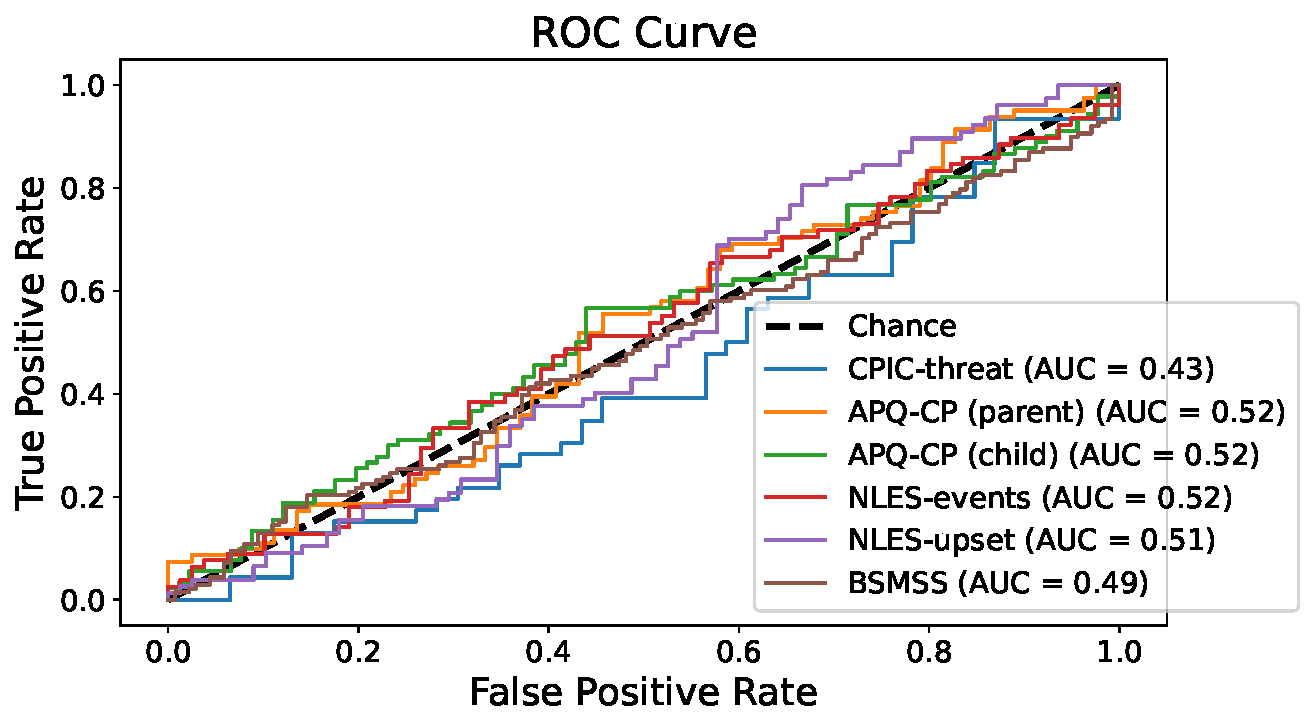
\includegraphics[width=\textwidth]{roc_curve_pcr_lasso.pdf}
        \captionof{figure}{
            Machine learning models fail to classify ELA exposure groups,
            yielding ROC curves that are similar to random guessing.
        }
    \end{Figure}

    \begin{center}
        There are no group differences in brain age gap.
    \end{center}

    \begin{Figure}
        \centering
        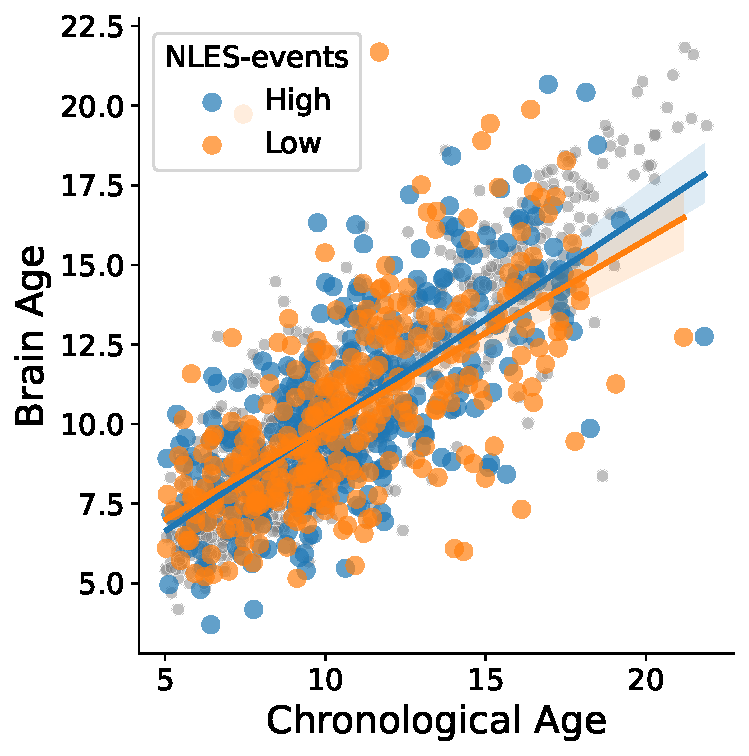
\includegraphics[width=0.475\textwidth]{bag-analysis-NLES-events.pdf}
        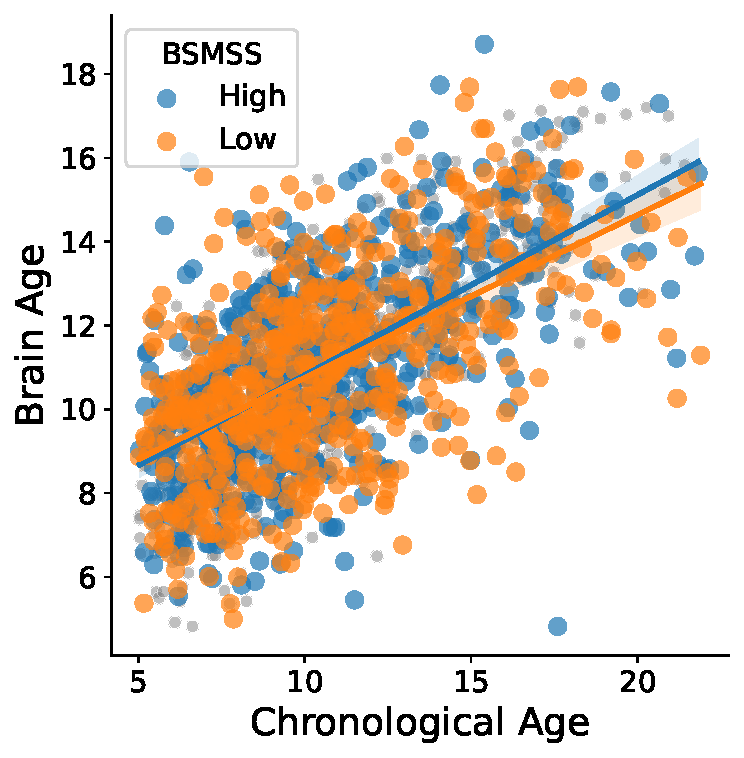
\includegraphics[width=0.475\textwidth]{bag-analysis-BSMSS.pdf}
        \captionof{figure}{
            ELA and SES groups exhibit no differences in brain age gap.
        }
    \end{Figure}
\end{minipage}
}

%----------------------------------------------------------------------------
%	Methods
%----------------------------------------------------------------------------

\headerbox{Methods}{name=methods,column=0,span=2,below=introduction,above=references}{

\begin{itemize}[nosep, leftmargin=*]
    \item ELA estimated using the self-reported negative life events scale (NLES).
    \item Threat dimension\cite{mclaughlin2014childhood} assessed using
    child perception of interparental conflict threat (CPIC-threat),
    Alabama parenting questionnaire corporal punishment (APQ-CP) subscales.
    \item These were binarized into ``low'' (below median) and ``high'' (upper
    tertile) groups.
    \item SES assessed using the Barratt simplified measure of social status (BSMSS).
    \item Confounding variables were statistically matched between target and
    normative cohorts.
\end{itemize}

\begin{minipage}[b]{0.68\textwidth}
    \begin{Figure}
        \centering
        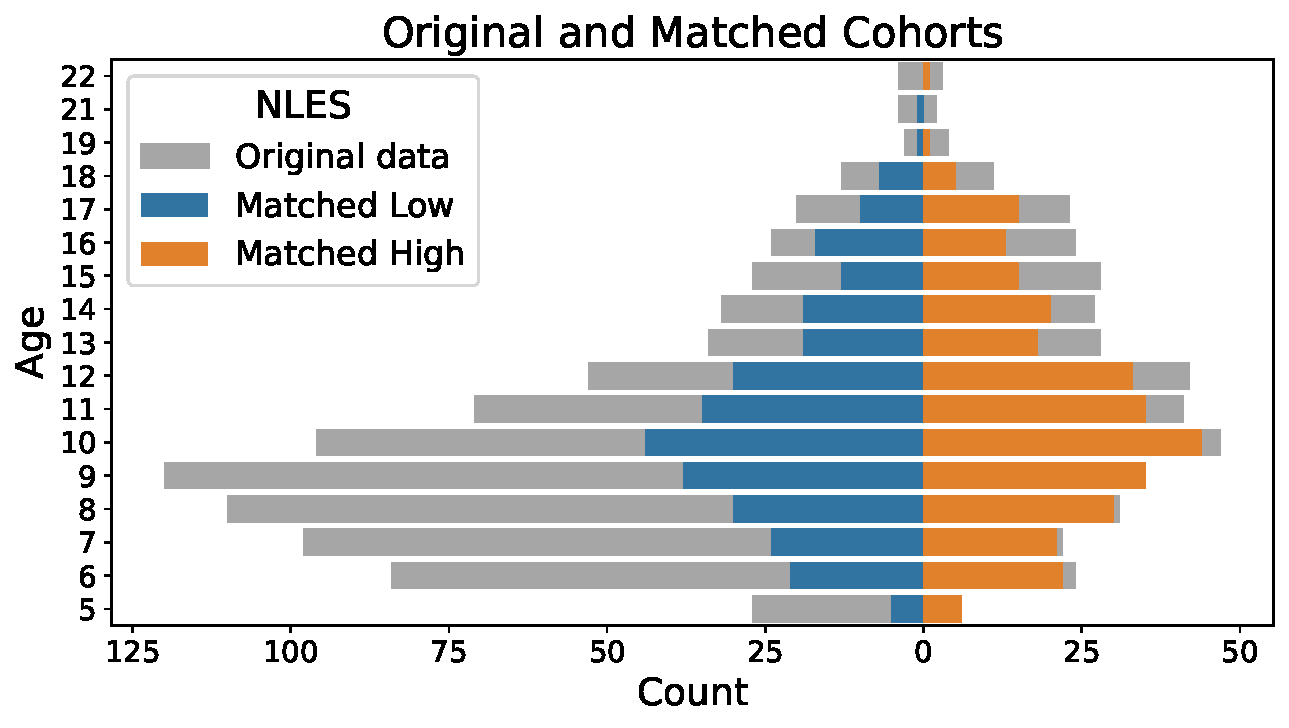
\includegraphics[width=\linewidth]{matching.pdf}
    \end{Figure}
\end{minipage}
\hfill
\begin{minipage}[b]{0.29\textwidth}
    \rowcolors{2}{white}{gray!25}
    \begin{tabular}{|p{2.1cm} p{0.95cm}|} 
        \hline
        Assessment & Cohort Size \\
        \hline\hline
        NLES-events & 628 \\
        NLES-upset & 620 \\
        APQ-CP \newline (parent) & 648 \\
        APQ-CP (child) & 724 \\
        CPIC-threat & 366 \\
        BSMSS & 1098 \\
        \hline
    \end{tabular}
    \vspace{2.7em}
\end{minipage}

\begin{itemize}[nosep, leftmargin=*]
    \item Group difference assessed \textbf{(1)} as a classification task using
    linear and non-linear machine learning (ML) models and \textbf{(2)} using brain age gap analysis
\end{itemize}

\begin{minipage}[b]{0.35\textwidth}
    \begin{Figure}
        \centering
        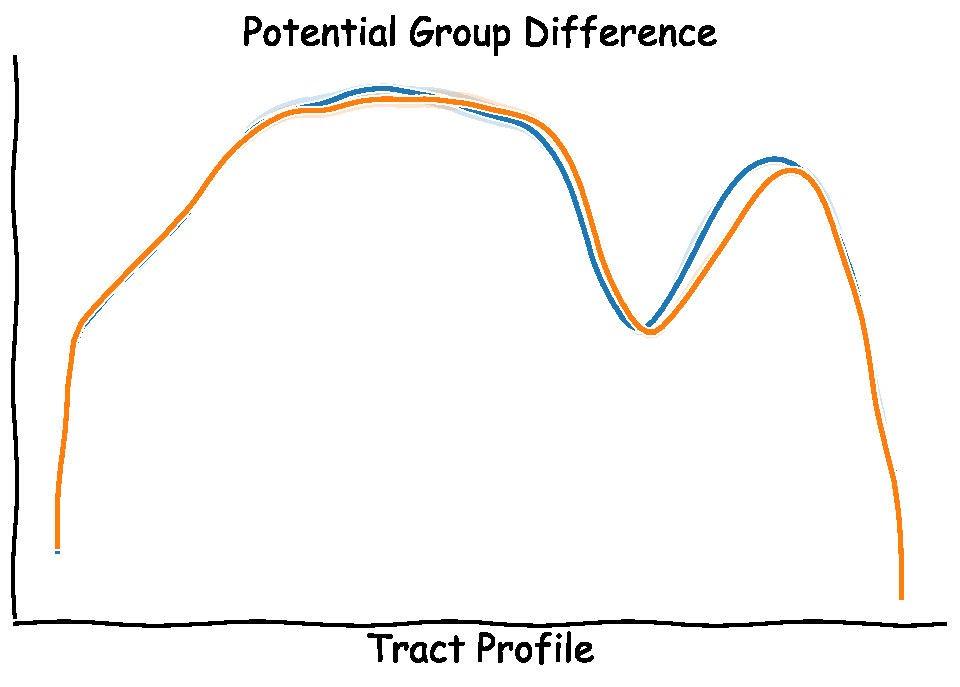
\includegraphics[width=\linewidth]{tract_profile_diff.pdf}
    \end{Figure}
\end{minipage}
\begin{minipage}[b]{0.05\textwidth}
    \centering
    $\Longrightarrow$
    \vspace{5em}
\end{minipage}
\begin{minipage}[b]{0.18\textwidth}
    \begin{Figure}
        \centering
        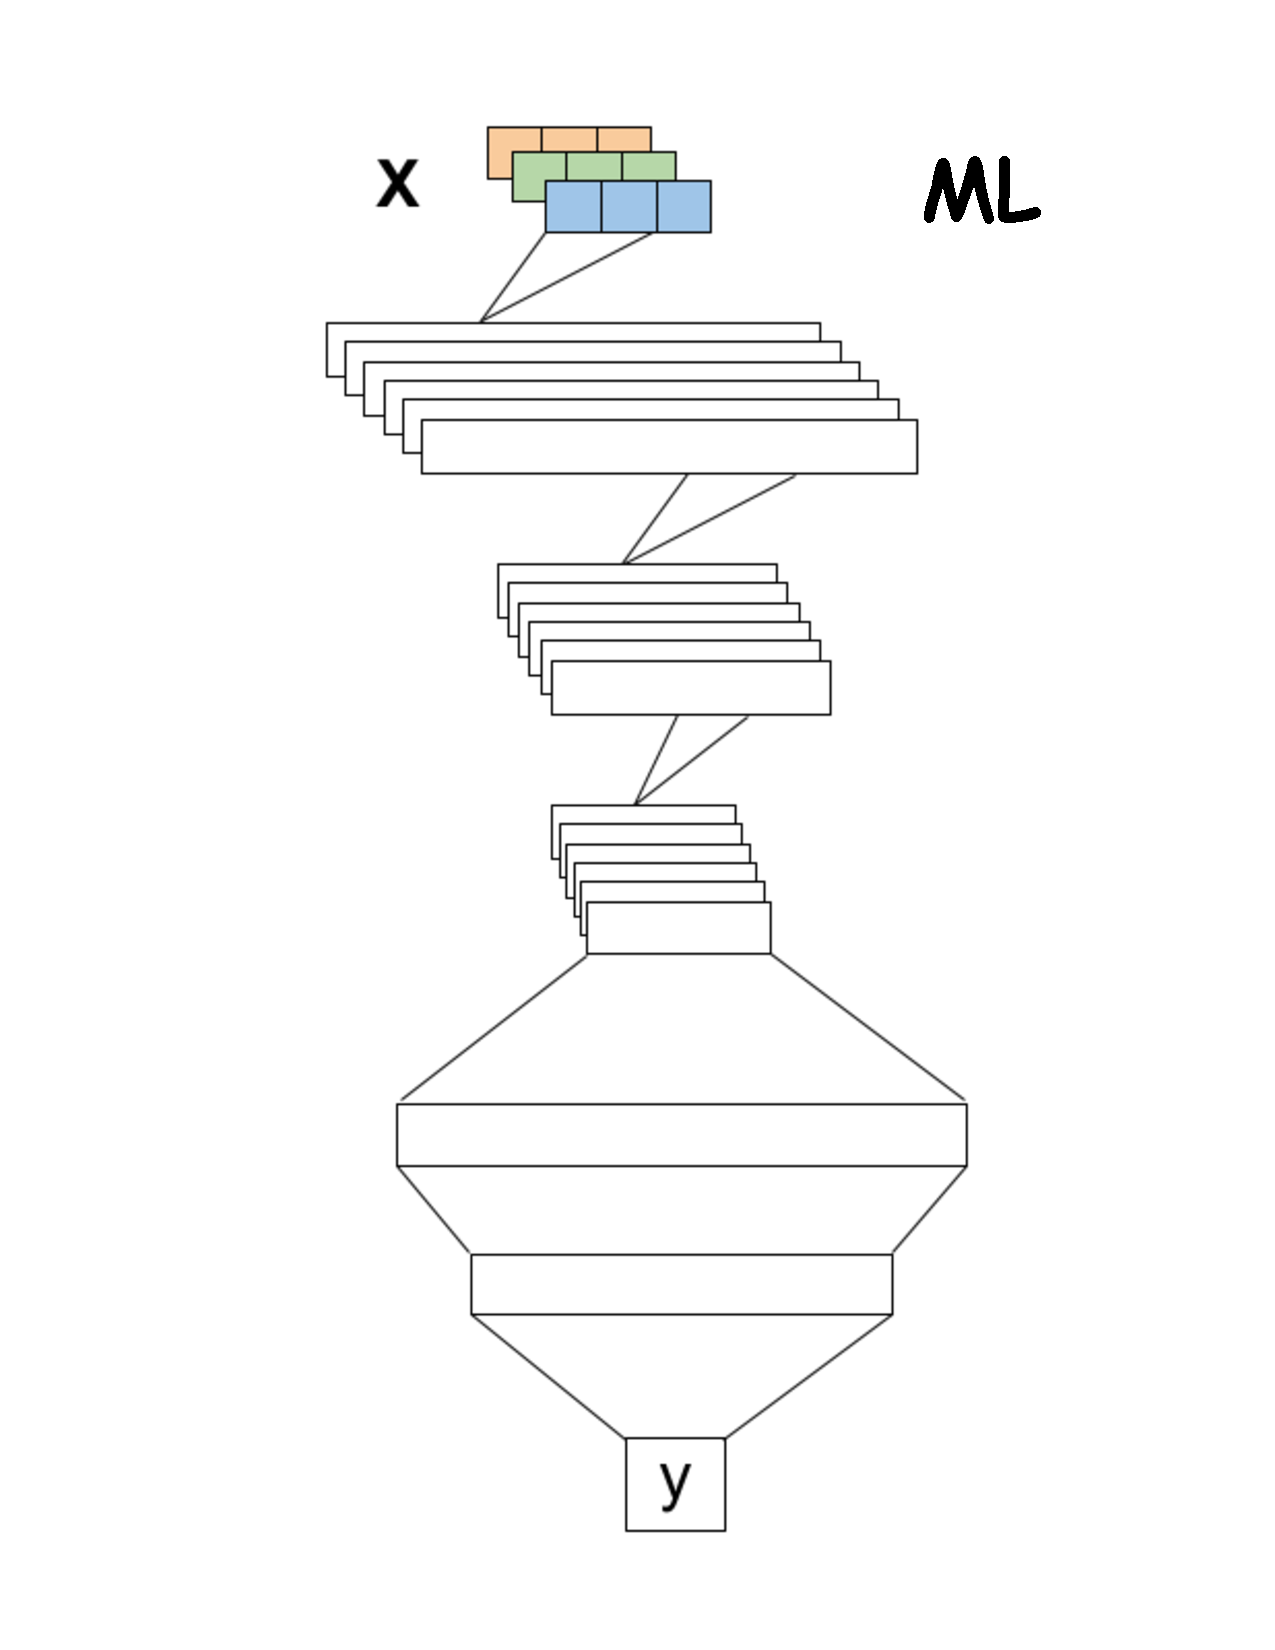
\includegraphics[width=0.75\linewidth]{convnet-schematic-1.pdf}
    \end{Figure}
\end{minipage}
\begin{minipage}[b]{0.05\textwidth}
    \centering
    $\Longrightarrow$
    \vspace{5em}
\end{minipage}
\begin{minipage}[b]{0.35\textwidth}
    \begin{Figure}
        \centering
        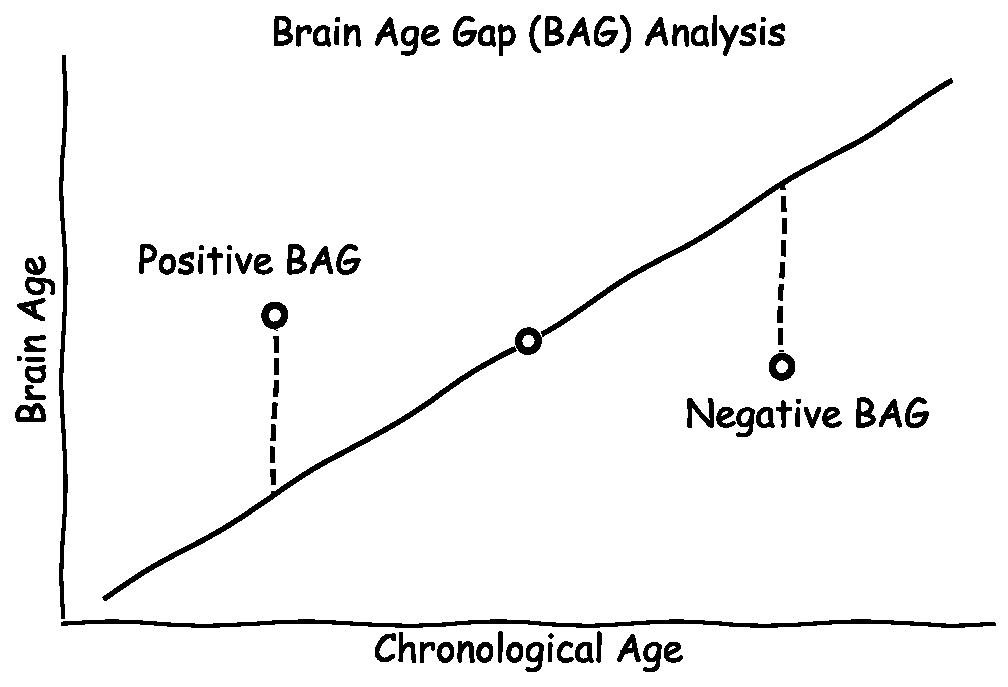
\includegraphics[width=\linewidth]{bag_analysis_cartoon.pdf}
    \end{Figure}
\end{minipage}
\vspace{-1em}
}

%----------------------------------------------------------------------------
%	DISCUSSION
%----------------------------------------------------------------------------

\headerbox{Discussion}{name=discussion,column=2,span=4,below=results}{

\begin{multicols}{2}
\begin{itemize}[nosep, leftmargin=*]
    \item \textbf{Finding}: we find no associations between exposure to early
    life adversity and white matter structure in the HBN dataset using three
    distinct methods
    \begin{itemize}[nosep, leftmargin=*]
        \item mass univariate statistical tests (p>0.05, FDR corrected for multiple comparisons)
        \item classification using advanced linear and non-linear models
        \item brain age gap (BAG) analysis
    \end{itemize}
    \item Limitations
    \begin{itemize}[nosep, leftmargin=*]
        \item As a self-reported, cumulative measure of ELA, NLES may be inadequate.
        \item Due to HBN's recruitment protocol, comorbidity with other
        psychopathologies is high.
        \item Cross-sectional data are inadequate to capture longitudinal
        changes due to ELA exposure.
    \end{itemize}
\end{itemize}
\end{multicols}
}

%----------------------------------------------------------------------------
%	ACKNOWLEDGMENTS
%----------------------------------------------------------------------------

\headerbox{Acknowledgments}{name=acknowledgments,column=4,span=2,below=discussion,above=bottom}{

\smaller % Reduce the font size in this block
\begin{minipage}[b]{0.70\textwidth}
\begin{minipage}[t]{0.31\textwidth}
    \centering
    
\includegraphics[height=1.0cm]{logos/nimh-logo.png}
    \newline {\normalsize 1RF1MH121868-01}
\end{minipage}
\hspace{1.5em} 
\includegraphics[height=1.1cm]{logos/SloanLogo.png}

\includegraphics[height=1.1cm]{logos/MooreFdn.png}
\hspace{6em} 
\includegraphics[height=1.1cm]{logos/eSciencelogo.png}
\end{minipage}
\hfill
\begin{minipage}[b]{0.13\textwidth}
    
\includegraphics[height=2.5cm]{qr.png}
\end{minipage}
}

%----------------------------------------------------------------------------
%   REFERENCES
%----------------------------------------------------------------------------

\headerbox{References}{name=references,column=0,span=4,below=discussion,above=bottom}{

\begin{multicols}{2}
\smaller \smaller % Reduce the font size in this block
\renewcommand{\section}[2]{\vskip 0.05em} % Get rid of the default "References" section title
\nocite{*} % Insert publications even if they are not cited in the poster

% \printbibliography
\bibliographystyle{unsrt85}
\bibliography{poster}
\end{multicols}
}

\end{poster}

\end{document}
